\chapter{2. Random variable generation}
\section{Introduction}
\subsection{The inverse transformation}
\begin{center}
\begin{marginfigure}
  \centering
  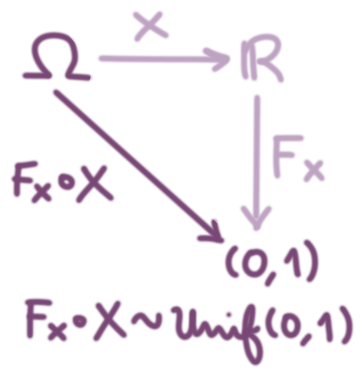
\includegraphics[scale=1]{26Feb_1.png}
\end{marginfigure}
\end{center}

\begin{teo}
\label{teo: inverse transf, teo 1}
(\textbf{p.44})
Sea $X$ una variable aletoria continua,
con funciones de densidad $f_{X}$ y $F_{X}$, respectivamente,
con $F_{X} : \IR \longrightarrow (0,1)$ invertible.
La variable aleatoria
\[
U=F_{X} \circ X
\]
tiene distribución $\mathcal{U}(0,1)$.
\end{teo}

\noindent
\textbf{Demostración.}
En efecto, sea $u \in (0,1)$. Puesto que por hipótesis
$F_{X}$ es invertible (o, equivalentemente,
biyectiva), existe un único $x \in \IR$ tal que
$F_{X}(x)=u$. Se tiene entonces que


\begin{align*}
P(U \leq u) = P (F_{X}(X) \leq F_{X}(x)) & =
P(F_{X}^{-1}(F_{X}(X)) \leq F_{X}^{-1}(F_{X}(X))) \\
= & P(X \leq x) = F_{X}(x)=u.
\end{align*}


\begin{figure}[H]
\centering
	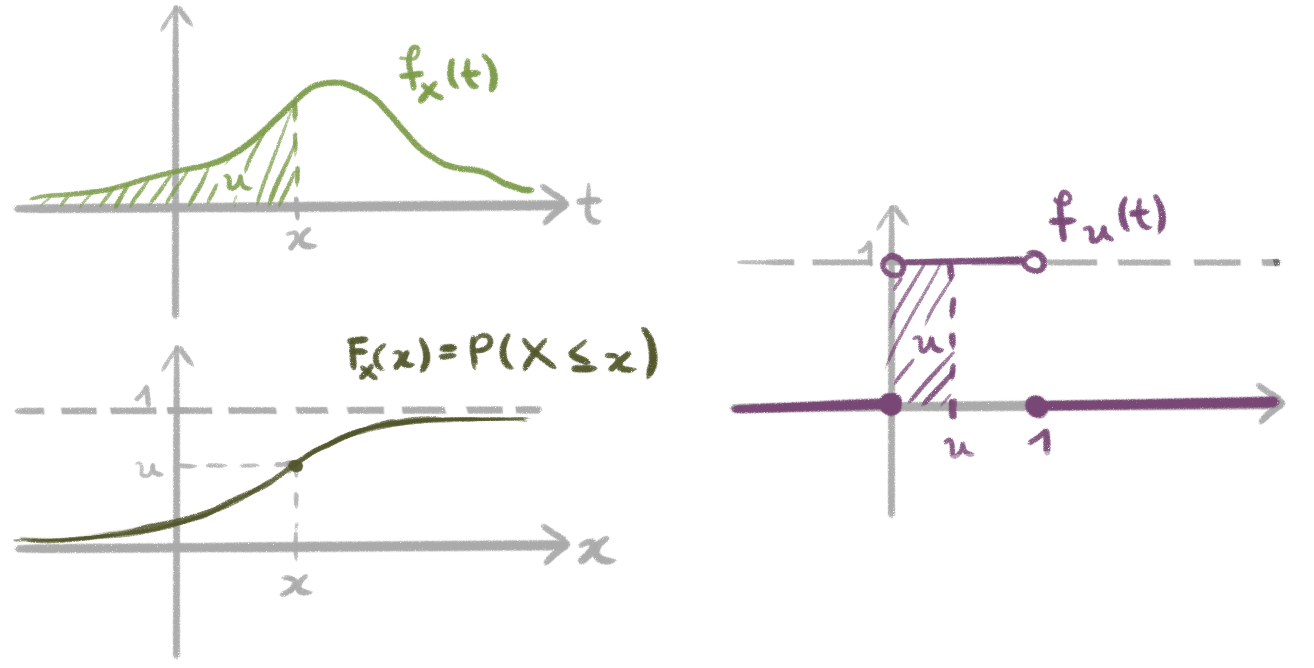
\includegraphics[scale=0.8]{26Feb_2} 
	\caption{a}
\end{figure}

\QEDB
\vspace{0.2cm}







El resultado dual se da a continuación.

\begin{center}
\begin{marginfigure}
  \centering
  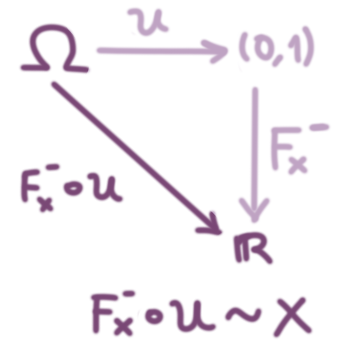
\includegraphics[scale=1]{26Feb_3.png}
\end{marginfigure}
\end{center}
\begin{ejercicio}
\label{ejerc: 2.1}
(\textbf{2.1, p.44})
Si $X$ es una variable aleatoria con función de
acumulación $F_{X}$, defina a la \textbf{inversa generalizada
de $F_{X}$} como sigue:

\begin{equation}
\label{ec: def inversa generalizada}
\forall u \in (0,1): \hspace*{0.2cm}
F_{X}^{-}(u):= inf\{x \hspace{0.1cm} : \hspace*{0.1cm} F_{X}(x) \geq u \}.
\end{equation}

Demuestre que si $U$ es una variable aleatoria con
distribución $U(0,1)$, entonces 
\[
F_{X}^{-} \circ U \sim X.
\]
\end{ejercicio}
\noindent
\textbf{Demostración.}

\begin{center}
\begin{marginfigure}
  \centering
  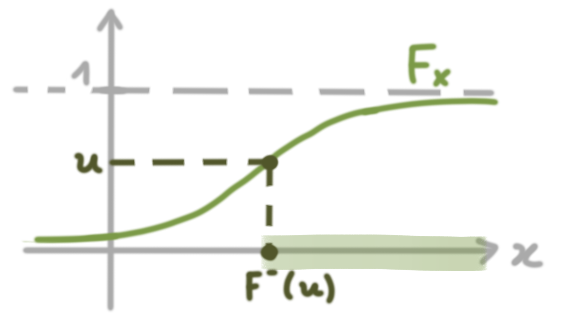
\includegraphics[scale=1]{26Feb_4.png}
  \caption{Definición de $F^{-}_{X}$.}
\end{marginfigure}
\end{center}


Sea $Y: \Om \longrightarrow \IR$ la composición
$F^{-}_{X} \circ U$. Debemos demostrar que

\begin{equation*}
\forall z \in \IR: \hspace*{0.2cm}
P(Y \leq z) = P(X \leq z).
\end{equation*}


Sea pues $z \in \IR$.

\begin{itemize}
\item[a)] Por ser $F_{X}$ una función de acumulación, es 
una función creciente, luego, los eventos
\[
(X \leq z) \hspace{0.2cm} \text{y} \hspace{0.2cm} 
(F_{X}(X) \leq F_{X}(z))
\]

son iguales; además, según el teorema 
\ref{teo: inverse transf, teo 1}, $F \circ X \sim U$; así,
\begin{equation}
\label{eq0: 26Feb}
P(X \leq z) = P(F_{X}(X) \leq F_{X}(z)) = P(U \leq F_{X}(z)).
\end{equation}

\item[b)] Por la definición de $F^{-}$ en términos de un 
ínfimo, se sigue de inmediato que
\begin{align*}
P(Y \leq z) = P(F^{-}_{X}(U) \leq z) = & 
P (\{w \in \Omega \hspace{0.1cm} : \hspace{0.1cm} F^{-}_{X}(U(w)) \leq z \}) \\
= & 
P (\{w \in \Omega \hspace{0.1cm} : \hspace{0.1cm} U(w) \leq F_{X}(z) \})
=P(U \leq F_{X}(z)),
\end{align*}

o sea, que 
\begin{equation}
\label{eq1: 26Feb}
P(Y \leq z) = P(U \leq F_{X}(z));
\end{equation}
\end{itemize}

de \eqref{eq0: 26Feb} y \eqref{eq1: 26Feb} se sigue,
como queríamos, que
$P(X \leq z) = P(Y \leq z)$.

\QEDB
\vspace{0.2cm}



\begin{ejercicio}
(\textbf{2.2, p. 45}) Se dan algunas funciones de probabilidad.
Calcule las correspondientes funciones de acumulación, y en base a
estas y los resultados anteriores, simule via una transformación
de variables aleatorias uniformes la distribución dada.
Comparar el resultado obtenido con las gráficas hechas
llamando a la distribución en R.
\end{ejercicio}

\noindent
\textbf{Solución}

\begin{itemize}
\item[a)] \textbf{Distribución logística}: la pdf es
\begin{equation}
\label{eq2: 26Feb}
f(x)= \frac{1}{\beta} \frac{e^{-(x- \mu)/ \beta}}{(1+e^{-(x- \mu)/ \beta})^{2}}
\end{equation}
(al parámetro $\mu$ se le llama \textbf{localización}, y al $\beta$
\textbf{escala}). Integrando, calculamos que

\[
\forall x \in \IR : \hspace{0.2cm}
F(x)= \frac{1}{1+e^{-(x-\mu)/\beta}};
\]
la inversa de esta función es 

\[
F^{-1}(u)= ln \left( \left( \frac{u}{1-u}  \right)^{\beta} \right) + \mu,
\]
luego, según el ejercicio \ref{ejerc: 2.1}, si $U \sim U(0,1)$, la variable
aleatoria
\[
Y = ln \left( \left( \frac{U}{1-U}  \right)^{\beta} \right) + \mu
\]
tiene a la función \eqref{eq2: 26Feb} como función de distribución.

Los valores de default de los parámetros de la distribución logística
en \texttt{rstudio} son 
\[
\mu=0, \hspace{0.2cm} \beta=1;
\]
a continuación comprobamos con un experimento numérico
en \texttt{rstudio} que las variables aleatorias
\begin{equation}
\label{eq3: 26Feb}
X = logistic(\mu=0, \beta=1) \hspace{0.2cm} \text{y}
\hspace{0.2cm} Y= ln \left( \frac{U}{1-U} \right)
\end{equation}
parecen tener la misma distribución.
\end{itemize}

\begin{figure}[H]
\centering
	\sidecaption{Histogramas de distribuciones logísticas
	(tamaño de muestra: $10^{4}$) usando las variables aleatorias
	\eqref{eq3: 26Feb}.}
	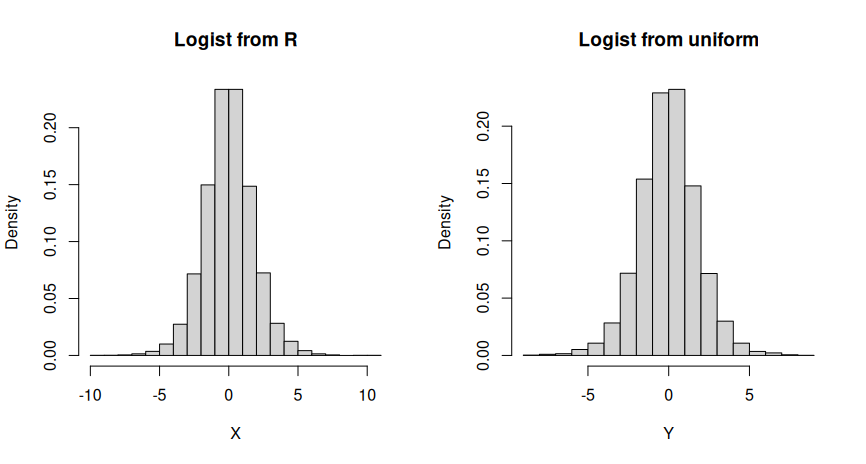
\includegraphics[scale=0.5]{logistic} 
\end{figure}
Código de R empleado para generar la imagen:
\begin{verbatim}
> Nsim=10^4
> U=runif(Nsim)
> X=rlogis(Nsim)
> Y=log(U/(1-U))
> par(mfrow=c(1,2))
> hist(X, freq=FALSE, main='Logist from R')
> hist(Y, freq=FALSE, main='Logist from uniform')
\end{verbatim}


\begin{itemize}
\item[b)] \textbf{Distribución de Cauchy}: la pdf es

\[
f(x)= \frac{1}{\pi \sigma} \frac{1}{1+ \left( \frac{x-\mu }{\sigma} \right)^{2}}.
\]
Después de integrar se llega a que 
\[
\forall x \in \IR : \hspace{0.2cm}
F(x)= \frac{1}{2} \frac{1}{\pi} arctan\left( \frac{x-\mu }{\sigma} \right).
\]

La inversa de esta transformación es 

\[
F^{-1}(u)= \mu + \sigma tan \left( \pi u -\frac{\pi}{2} \right),
\hspace{0.2cm} 0 < u < 1,
\]
luego, 
según el ejercicio \ref{ejerc: 2.1}, si $U \sim U(0,1)$, la variable
aleatoria
\[
F^{-1}(U)= \mu + \sigma tan \left( \pi U -\frac{\pi}{2} \right)
\]
tiene distribución de Cauchy con parámetros $\mu$ y $\sigma$.

Haciendo $\mu=0$ y $\sigma=1$, podemos graficar los histogramas
de $10^4$ variables aleatorias


\begin{equation}
\label{eq0: 2Marz}
X \sim Cauchy (\mu, sigma), \hspace{0.2cm} \text{y}
\hspace{0.2cm} Z= \mu + \sigma tan \left( \pi U -\frac{\pi}{2} \right)
\end{equation}


y compararlos; como se ve en la figura, resultado de correr
el código de más abajo, estos histogramas son casi idénticos.
\end{itemize}



\begin{figure}[H]
\centering
	\sidecaption{Histogramas de distribuciones Cauchy
	(tamaño de muestra: $10^{4}$) usando las variables aleatorias
	\eqref{eq0: 2Marz}.}
	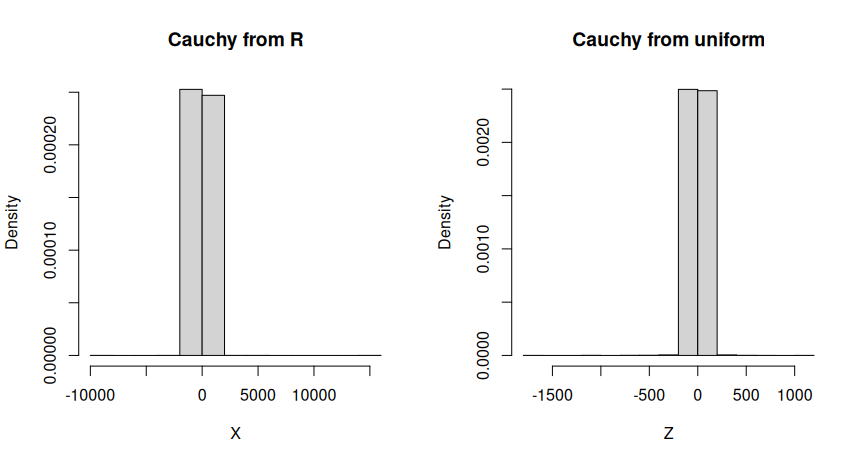
\includegraphics[scale=0.5]{CauchyFromUnif} 
\end{figure}

Código de R empleado para generar la imagen:
\begin{verbatim}
> Nsim=10^4
> U=runif(Nsim)
> X=rcauchy(Nsim)
> Z=tan(3.1416*(U-0.5))
> par(mfrow=c(1,2))
> hist(X, freq=FALSE, main='Cauchy from R')
> hist(Z, freq=FALSE, main='Cauchy from uniform')
\end{verbatim}
\vspace{0.2cm}



\subsection{2.2: General transformation methods}

Según un ejemplo del libro, si $U \sim U(0,1)$, entonces
$-ln(U) \sim Exp(1)$. Se establecen además las siguientes
relaciones:

\begin{teo}
Sea $\{ X_{i} \}_{i \in \mathbb{N}}$ iid $Exp(1)$ variables aleatorias.
Para cualesquiera $a, b, v \in \mathbb{N}2^{*}$, 

\begin{equation}
\label{eq1: 2Marz}
Y=2 \suma{j=1}{v}{X_{j}} \sim \chi_{2v}^{2},
\end{equation}

\begin{equation}
\label{eq2: 2Marz}
Y=\beta \suma{j=1}{a}{X_{j}} \sim \mathcal{G}(a, \beta),
\end{equation}

\begin{equation}
\label{eq3: 2Marz}
Y= \frac{\suma{j=1}{a}{X_{j}}}{\suma{j=1}{a+b}{X_{j}}} 
\sim Beta(a,b).
\end{equation}
\end{teo}

Comprobemos las fórmulas \eqref{eq1: 2Marz}, \eqref{eq2: 2Marz}
y \eqref{eq3: 2Marz} con algunas simulaciones en R.

\begin{center}
\begin{marginfigure}
  \centering
  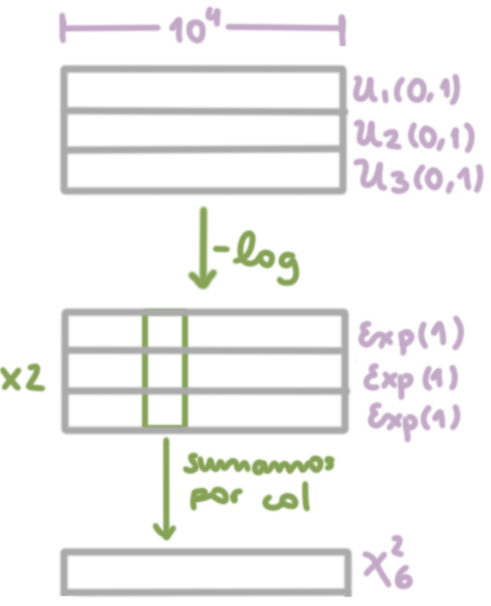
\includegraphics[scale=1]{2Marz.png}
  \caption{Explicación gráfica del proceso de simulación.}
\end{marginfigure}
\end{center}

\begin{verbatim}
> U=runif(3*10^4)
> U=matrix(data=U, nrow=3)
> X=-log(U)
> Y=2*apply(X, 2, sum)
> Z=rchisq(10^4, df=6)
> par(mfrow=c(1,2))
> hist(Z, freq=FALSE, main='Chi df=6 from R')
> hist(Y, freq=FALSE, main='Chi df=6 from Exp')
\end{verbatim}

\begin{figure}[H]
\centering
	\sidecaption{Histogramas de $Y=2(X_{1}+X_{2}+X_{3})$, con $X_{i}$,
	$1 \leq i \leq 3$ iid $Exp(1)$ y de $Z \sim \chi^{2}_{6}$. }
	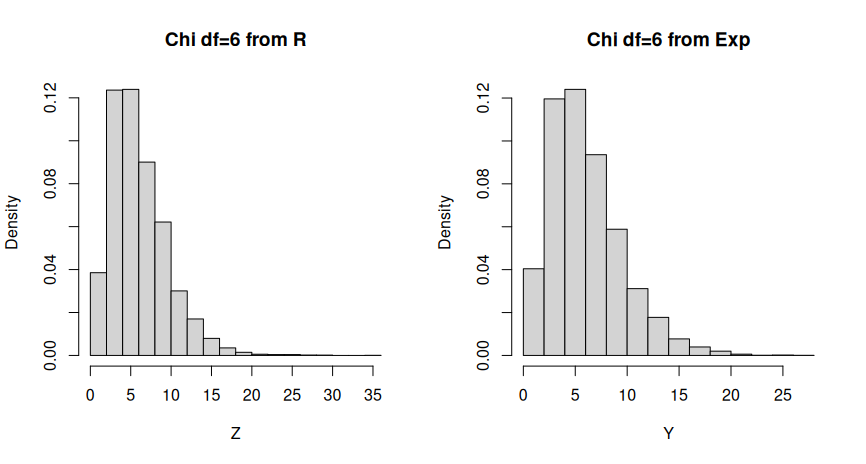
\includegraphics[scale=0.5]{chiFromExp} 
\end{figure}

\TODO{No pude simular correctamente las otras dos distribuciones!}
\subsection{2.2.1 A normal generator}
\begin{teo}
\textbf{(Box-Muller)} if $U_{1}$ and $U_{2}$ are iid uniforms in $]0,1[$,
then the variables
\[
X_{1} := \sqrt{-2 log(U_{1})} cos(2 \pi U_{2})
\]
and 
\[
X_{2} := \sqrt{-2 log(U_{1})} sen(2 \pi U_{2})
\]
are iid N(0,1).
\end{teo}

\begin{verbatim}
> n = 10**4
> U1 = runif(n)
> U2 = runif(n)
> X1 = sqrt(-2*log(U1))*cos(2*pi*U2)
> X2 = sqrt(-2*log(U1))*sin(2*pi*U2)
> N = rnorm(n,0,1)
> par(mfrow=c(1,3))
> hist(X1, freq=FALSE, main='Primera normal de BM')
> hist(X2, freq=FALSE, main='Segunda normal de BM')
> hist(N, freq=FALSE, main='Normal de R')
\end{verbatim}
\begin{figure}[H]
	\sidecaption{
	Usamos el algoritmo de Box-Muller para generar dos normales estandar.
	Comparamos sus histogramas con el de una normal generada por R.
	\label{fig: BM}
	}
	\centering
	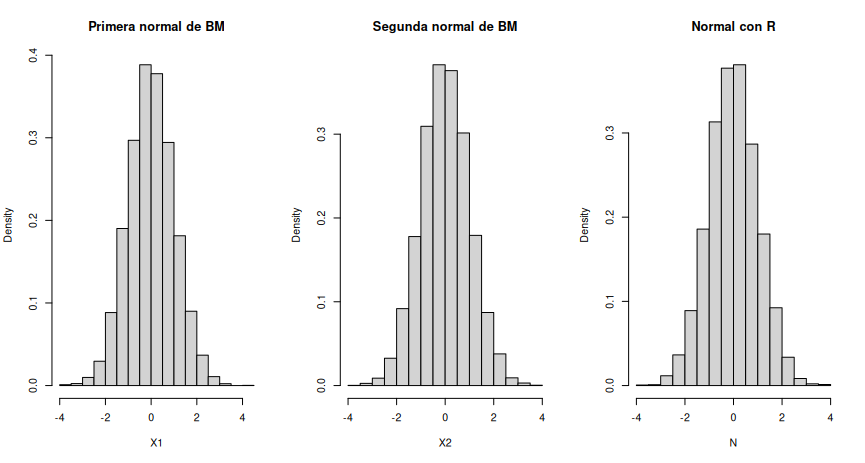
\includegraphics[scale=0.55]{BM} 
\end{figure}	

\begin{figure}[H]
	\sidecaption{
	\label{fig: BM explained}
	}
	\centering
	\includegraphics[scale= 1]{Box-Muller} 
\end{figure}	

\begin{ejercicio}
\textbf{(2.3)} Podemos usar el \textbf{teorema del 
límite central} para generar una distribución normal a partir de 
variables aleatorias uniformes e independientes. \\

Sean $U_{i} \sim U[-1/2, 1/2]$, $0 \leq i \leq 12$.
Se calcula que, para toda $i$, $E[U_{i}]=0$ y
$Var[U_{i}] = 1/12$.
Si $Z := \suma{i=1}{12}{U_{1}}$, entonces
\[
E(Z) = \suma{i=1}{12}{E(U_{i})} = 0
\]
y 
\[
Var(Z) = \suma{i=1}{12}{Var(U_{i})} = 1;
\]

\noindent
ahora bien, según el TLC, la variable aleatoira
\[
\frac{Z - E(Z)}{\sqrt{Var(Z)}} = Z
\]
tiende en probabilidad a $N(0,1)$
\begin{verbatim}
> n = 10**4
> Z1 = rnorm(n, 0, 1)
> U =runif(12*10**4)
> U = matrix(data = U, nrow=12)
> Z2 = apply(U, 2, sum)
> U1 = runif(n)
> U2 = runif(n)
> Z3 = sqrt(-2*log(U1))*cos(2*pi*U2)
> par(mfrow=c(1,3))
> hist(Z1, freq = FALSE, main = "Normal con R")
> hist(Z2, freq = FALSE, main = "Normal con TLC")
> hist(Z3, freq = FALSE, main = "Normal con BM")
\end{verbatim}
\end{ejercicio}
\begin{figure}[H]
	\sidecaption{
	Resultados de las simulaciones en R.
	Por lo general se prefire usar BM a TLC, pues
	el primero da lugar a v.a. que en efecto tienen
	distribuciones $N(0,1)$, mientras que el segundo
	método siempre da aproximaciones.
	\label{fig: generadores_normal}
	}
	\centering
	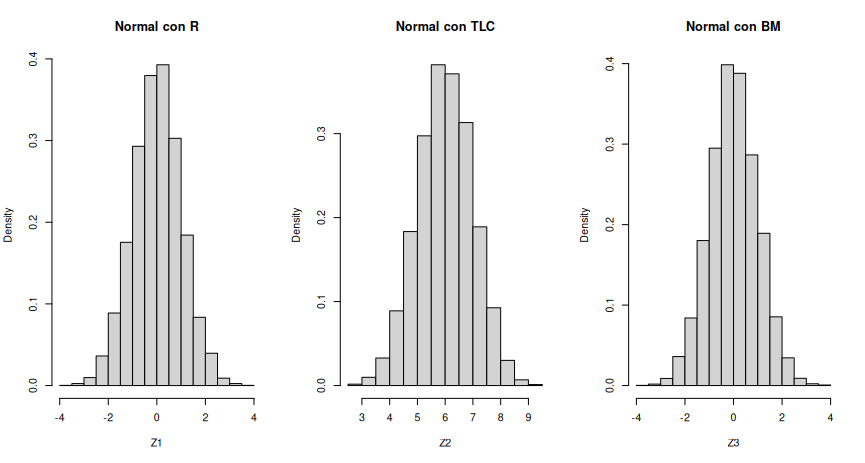
\includegraphics[scale= 0.55]{generadores_normal} 
\end{figure}	

\subsection{2.2.2 Discrete distributions}

A partir de una variable uniforme
$U \sim U(0,1)$, también es posible generar distribuciones
discretas. Sea $P_{\theta}$ una distribución cuyo 
soporte está contenido en $\mathbb{Z}$, y sea
$X \sim P_{\theta}$.


Calcular a $F_{\theta}$ (la función de acumulación
de la distribución) se reduce a calcular 
(\textbf{y, en la práctica, guardar en la memoria})
los siguientes números;

\begin{equation}
\label{eq0: 20Ap}
p_{k} := P(X \leq k)
\end{equation}

\begin{figure}[H]
	\sidecaption{
	Recuerde cómo se define la inversa generalizada
	de la función de acumulación $F$ en 
	\eqref{ec: def inversa generalizada}.
	\label{fig: 20ap 1}
	}
	\centering
	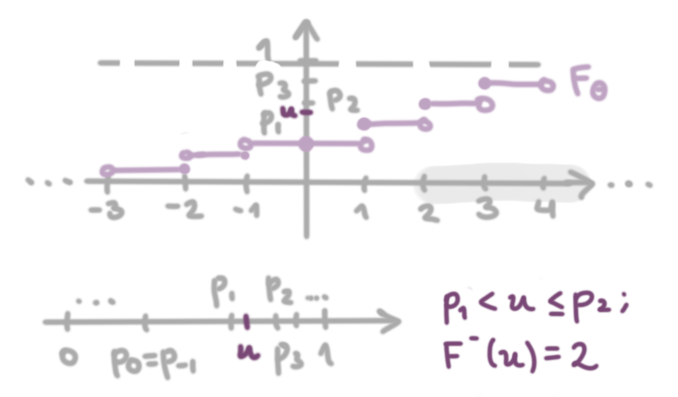
\includegraphics[scale= 1.3]{20ap_1} 
\end{figure}	

La inversa generalizada $F_{\theta}^{-}$ de la función
de acumulación dada es
\[
\aplica{F_{\theta}^{-}}{]0,1[}{\{ p_{k} \}_{k \in \mathbb{Z}} }{u}{
k \hspace{0.2cm} \textit{si } p_{k-1} < u \leq p_{k}.
}
\]

Según el ejercicio \ref{ejerc: 2.1},
$X:= F^{-}_{\theta} \circ U \sim P_{\theta}$.

\TODO{checa cómo tienes los environments de ejemplo en tu tesis.}
\begin{ej}
Este es el resultado de usar las ideas de esta sección para,
a partir de números aleatorios de una distribución
$U(0,1)$, obtener una distribución binomial.
\end{ej}
\begin{figure}[H]
	\sidecaption{
	Figura generada usando el
	código de \texttt{generar$\_$binomial.py}
	\label{fig: binom de unif}
	}
	\centering
	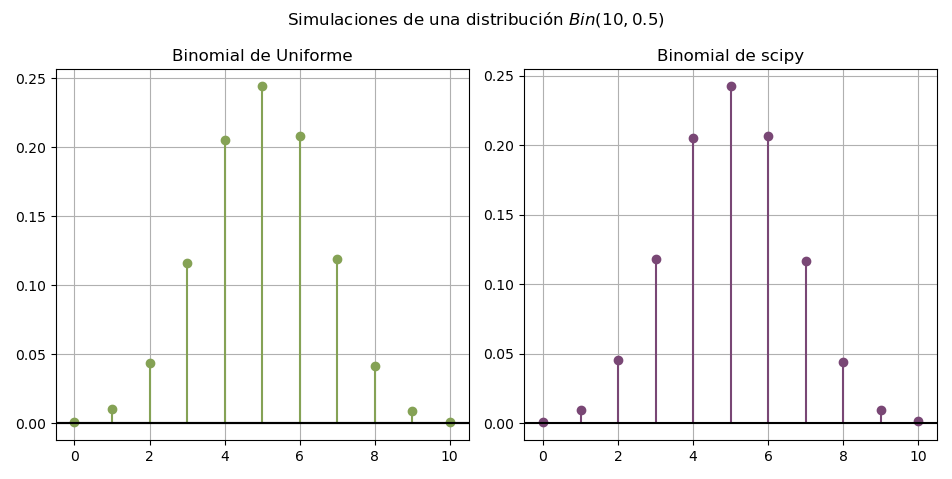
\includegraphics[scale = 0.5]{binom_de_unif} 
\end{figure}	

\begin{figure}[H]
	\sidecaption{
	Figura generada usando el
	código de \texttt{generar$\_$binomial.py}
	\label{fig: binom de unif}
	}
	\centering
	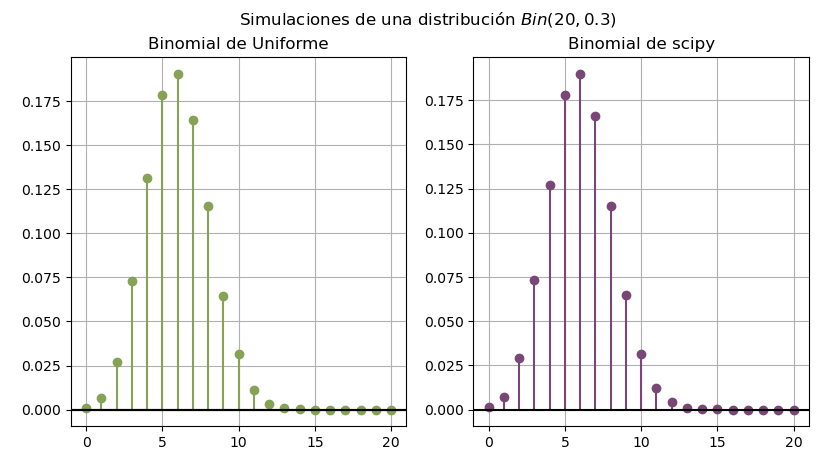
\includegraphics[scale = 0.5]{binom_de_unif_2} 
\end{figure}	

Vamos a hacer lo mismo pero ahora con \texttt{R}.

\begin{verbatim}
> Nsim = 10^4; n = 10; p = 0.3
> soporte = seq(0, n, 1)
> vector_pk = pbinom(soporte, n, p)
> X = rep(0, Nsim) 
> for (i in 1:Nsim){
+ u = runif(1)
+ X[i] = sum(vector$\_$pk<u)
+ }
\end{verbatim}
Note que \texttt{vector$\_$pk} es el vector en el que
se almacenan los valores $p\_{k}$ para
$0 \leq k \leq n$ (que, en el caso de la distribución
binomial, son todos los valores de $k$ que basta considerar),
y que \texttt{vector$\_$pk} es un vector de booleanos,
cuya $i-$ésima entrada es \texttt{TRUE} si la i-ésima
entrada de \texttt{vector$\_$pk} es menor a $u$, y es 
\texttt{FALSE} en caso contrario. Nota entonces que
$\texttt{sum(vector\_pk<u)} = F^{-}(u)$. 
